\documentclass{article}
\usepackage[utf8]{inputenc}
\usepackage{xcolor}
\usepackage{amsmath}
\usepackage{amsfonts, amssymb}
\usepackage{natbib}
\usepackage{url}
\usepackage{graphicx}
\usepackage{hyperref}
\usepackage{authblk}
\usepackage{booktabs}
\usepackage{longtable}
\usepackage{listings}
\usepackage{geometry}
\usepackage{tikz}
\usetikzlibrary{shapes.geometric, arrows.meta, positioning, fit}

\geometry{margin=1in}

\bibliographystyle{plainnat}

\newcommand{\HRule}{\rule{\linewidth}{0.5mm}}

\lstset{
  basicstyle=\ttfamily\small,
  breaklines=true,
  frame=single,
  language=SQL,
  keywordstyle=\color{blue},
  commentstyle=\color{gray},
  stringstyle=\color{red},
  showstringspaces=false
}

\begin{document}
\begin{titlepage}

\center
\textbf{}\\[2cm]

\textsc{}{\LARGE 02360323 -- Project in Data Processing}\\[1cm]
\par\noindent\rule{\textwidth}{0.3pt} \\[0.8cm]
{\huge \bfseries Entity Resolution Dataset Construction\\[0.3cm] for RelBench}\\[0.7cm]
\par\noindent\rule{\textwidth}{0.3pt} \\[1.5cm]

\textbf{\huge Yuval Lubarsky \footnote{lubarsky@cs.technion.ac.il, ID -- 208001990}}\\[1cm]
\textbf{\LARGE Advisor: Prof. Benny Kimelfeld}\\[1cm]

\LARGE March 2026 \\
\textsc{}


\includegraphics[width=0.5\textwidth]{technion.jpg}
\vfill
\end{titlepage}


\tableofcontents
\newpage


%======================================================================
\section{Introduction}
%======================================================================

Entity Resolution (ER) is one of the oldest and most practical problems in data management.
The idea is simple: given records from one or more data sources, figure out which records refer to the same real world entity.
For example, the paper ``Attention Is All You Need'' might appear as one record in DBLP and as a different record in Semantic Scholar, with slightly different metadata, different IDs, and maybe a different title format.
ER is the task of linking these two records together.

Despite decades of research, most ER benchmarks consist of small, two table datasets.
Amazon vs.\ Google Products, Abt vs.\ Buy, and similar benchmarks from the Magellan repository have been the standard for years.
These are useful for quick evaluation, but they do not reflect the complexity of real world data integration scenarios where you have multiple interconnected tables, millions of records, and rich relational structure (citations, authorship, venues, etc.).

Recently, the RelBench framework \citep{robinson2024relbench} introduced a new paradigm: Relational Deep Learning (RDL).
The idea is to represent relational databases as heterogeneous graphs and use Graph Neural Networks (GNNs) to learn directly from the multi table structure, without manual feature engineering.
RelBench comes with several benchmark datasets (Amazon reviews, Stack Overflow, Formula 1, and others), but at the time of this project it did not include a large scale Entity Resolution task.

The goal of this project was to fill that gap.
I built a large ER dataset by combining two major bibliographic databases: DBLP and Semantic Scholar.
The dataset contains millions of papers, authors, citations, and abstracts spread across multiple relational tables.
I also defined a ground truth for the matching task and integrated everything into RelBench as a custom dataset and task.

To be clear about what this project is and is not: the main contribution is the dataset construction pipeline.
I did not develop new ER algorithms or train state of the art models.
What I did do is all the data engineering work needed to create a usable, large scale, multi table ER benchmark, from scraping and downloading the raw data, to cleaning it, setting up a PostgreSQL database, generating ground truth, enforcing referential integrity, and packaging it for RelBench.
I also ran a small proof of concept experiment on a subset of the data to show that the dataset works with RelBench's GNN and LightGBM training pipelines.

The rest of this report is organized as follows.
Section~\ref{sec:background} covers the background on ER, RelBench, and the data sources.
Section~\ref{sec:related} reviews related work.
Section~\ref{sec:dataset} describes the dataset construction process in detail.
Section~\ref{sec:relbench} explains how the dataset was integrated into RelBench.
Section~\ref{sec:experiments} presents the proof of concept experiment.
Section~\ref{sec:limitations} discusses limitations, and Section~\ref{sec:conclusion} concludes.


%======================================================================
\section{Background}
\label{sec:background}
%======================================================================

\subsection{Entity Resolution}

Entity Resolution is the process of identifying records that refer to the same real world entity.
It goes by many names in the literature: record linkage, deduplication, entity matching, and data matching.
The general ER pipeline has two main phases:

\begin{enumerate}
    \item \textbf{Blocking}: Reduce the number of candidate pairs by grouping records into blocks based on some cheap similarity criterion. Without blocking, you would need $O(n^2)$ comparisons which is impractical for large datasets.
    \item \textbf{Matching}: For each candidate pair, determine whether the two records refer to the same entity. This can be done with rules, traditional ML classifiers, or more recently with deep learning models.
\end{enumerate}

Classical approaches use string similarity measures (Jaccard, edit distance, TF-IDF) on attribute values.
More recent work applies deep learning: DeepMatcher \citep{mudgal2018deepmatcher} uses attention based architectures, Ditto \citep{li2020ditto} fine tunes pre-trained language models for matching, and several works explore GNN based approaches \citep{loster2021grapher, yao2022hiergat}.

An important observation from \citet{bhattacharya2007collective} is that ER can benefit from relational structure: if two papers share the same co-authors or cite the same references, that is evidence they might be the same paper.
This idea of collective ER is particularly relevant for our dataset, which has rich relational structure.

\subsection{RelBench and Relational Deep Learning}

RelBench \citep{robinson2024relbench} is a benchmark framework for deep learning on relational databases.
The core idea, introduced in \citet{fey2024relational}, is Relational Deep Learning (RDL): represent a relational database as a temporal heterogeneous graph, where each row in each table becomes a node, and primary key / foreign key links become edges.
A GNN can then learn representations that capture the full relational structure, without any manual feature engineering.

RelBench provides:
\begin{itemize}
    \item A \texttt{Dataset} abstraction that wraps a relational database with train/validation/test temporal splits.
    \item A \texttt{Task} abstraction that defines prediction tasks (node classification, regression, link prediction).
    \item Graph construction utilities that convert the relational schema into a PyTorch Geometric heterogeneous graph.
    \item Example training scripts using GNN models (HeteroGraphSAGE) and baselines (LightGBM).
\end{itemize}

Each dataset defines tables with primary keys, foreign keys, and optional time columns.
The time columns enable temporal splitting: the model trains only on data up to the validation timestamp and is evaluated on future data, which prevents data leakage.

\subsection{DBLP}

DBLP \citep{ley2009dblp} is a comprehensive bibliography for computer science publications.
It provides structured metadata for over 6 million publications, including articles, conference papers (inproceedings), books, and theses.
The data is available as a large XML dump and through a public API.
Each record has a unique key (e.g., \texttt{conf/nips/VaswaniSPUJGKP17}) that serves as a persistent identifier.

For this project, I used the XML dump and parsed it into relational tables: publications, articles, inproceedings, books, incollections, authors, and an authorship relation.

\subsection{Semantic Scholar}

Semantic Scholar \citep{kinney2023semantic} is an AI powered academic search engine maintained by the Allen Institute for AI.
Its open data platform provides access to metadata for over 200 million papers from across all scientific disciplines.
The data is available through a REST API and through bulk downloads of the S2ORC corpus \citep{lo2020s2orc}.

A key feature for this project is that Semantic Scholar records often contain external identifiers, including DBLP keys, in their \texttt{externalIds} field.
This cross reference is what I used to build the ground truth for the ER task.


%======================================================================
\section{Related Work}
\label{sec:related}
%======================================================================

\paragraph{ER Benchmarks.}
The most commonly used ER benchmarks are relatively small.
Amazon vs.\ Google Products, Abt vs.\ Buy, and the WDC Products corpus are the standard evaluation datasets.
\citet{primpeli2023critical} showed that many of these benchmarks are actually too easy for modern deep learning methods and proposed new, more challenging datasets.
However, even these new datasets typically consist of just two flat tables.
There is a gap in the literature for large, multi table ER benchmarks with rich relational structure.

\paragraph{Deep Learning for ER.}
DeepMatcher \citep{mudgal2018deepmatcher} was among the first to apply deep learning to entity matching.
Ditto \citep{li2020ditto} showed that fine tuning pre-trained language models (like BERT) can achieve strong results.
HierGAT \citep{yao2022hiergat} uses hierarchical graph attention to model interdependence between ER decisions.
GraphER \citep{loster2021grapher} combines graph differential dependencies with GNNs for ER on property graphs.
FlexER \citep{sagi2022flexer} addresses the problem of multiple intents in ER using a multiplex graph representation, which is closely related to our setting where the same entity can appear with different roles across sources.

\paragraph{Blocking Methods.}
The blocking phase is critical for scalability.
\citet{papadakis2019blocking} provide a comprehensive survey of blocking and filtering techniques.
DeepBlocker \citep{thirumuruganathan2021deepblocker} explores deep learning for blocking.
SC-Block \citep{scblock2023} uses supervised contrastive learning for efficient blocking.
\citet{papadakis2023pretrained} provide an experimental analysis of pre-trained embeddings for both blocking and matching.

\paragraph{Relational Deep Learning.}
The RelBench benchmark \citep{robinson2024relbench} and the RDL framework \citep{fey2024relational} are directly relevant to this project.
Recent extensions include RelGNN \citep{relgnn2025}, which introduces composite message passing specifically designed for relational database graphs.


%======================================================================
\section{Dataset Construction}
\label{sec:dataset}
%======================================================================

This section describes the full pipeline for building the ER dataset.
The process took several months and many iterations.
Figure~\ref{fig:pipeline} shows a high level overview.

\begin{figure}[h!]
\centering
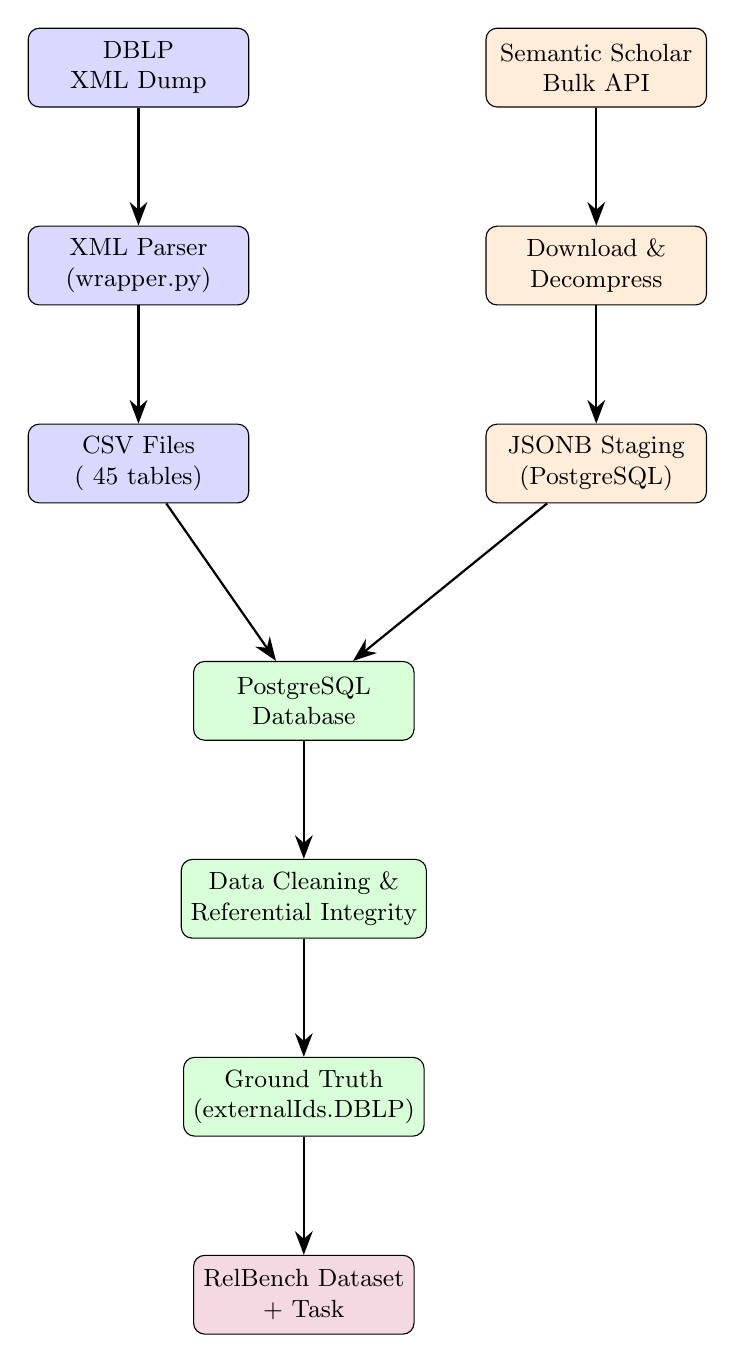
\begin{tikzpicture}[
    box/.style={rectangle, draw, rounded corners, minimum width=2.8cm, minimum height=1cm, align=center, font=\small},
    arrow/.style={-{Stealth[length=3mm]}, thick},
    node distance=1.5cm
]
    % DBLP side
    \node[box, fill=blue!15] (dblp_xml) {DBLP\\XML Dump};
    \node[box, fill=blue!15, below=of dblp_xml] (dblp_parse) {XML Parser\\(wrapper.py)};
    \node[box, fill=blue!15, below=of dblp_parse] (dblp_csv) {CSV Files\\(~45 tables)};

    % Semantic Scholar side
    \node[box, fill=orange!15, right=3cm of dblp_xml] (s2_api) {Semantic Scholar\\Bulk API};
    \node[box, fill=orange!15, below=of s2_api] (s2_download) {Download \&\\Decompress};
    \node[box, fill=orange!15, below=of s2_download] (s2_json) {JSONB Staging\\(PostgreSQL)};

    % Merge
    \node[box, fill=green!15, below=2cm of dblp_csv, xshift=2.1cm] (postgres) {PostgreSQL\\Database};
    \node[box, fill=green!15, below=of postgres] (clean) {Data Cleaning \&\\Referential Integrity};
    \node[box, fill=green!15, below=of clean] (ground) {Ground Truth\\(externalIds.DBLP)};
    \node[box, fill=purple!15, below=of ground] (relbench) {RelBench Dataset\\+ Task};

    % Arrows
    \draw[arrow] (dblp_xml) -- (dblp_parse);
    \draw[arrow] (dblp_parse) -- (dblp_csv);
    \draw[arrow] (dblp_csv) -- (postgres);

    \draw[arrow] (s2_api) -- (s2_download);
    \draw[arrow] (s2_download) -- (s2_json);
    \draw[arrow] (s2_json) -- (postgres);

    \draw[arrow] (postgres) -- (clean);
    \draw[arrow] (clean) -- (ground);
    \draw[arrow] (ground) -- (relbench);
\end{tikzpicture}
\caption{Overview of the dataset construction pipeline. DBLP data is parsed from XML, Semantic Scholar data is downloaded via the bulk API and staged as JSONB in PostgreSQL. Both sources are cleaned and linked through the ground truth.}
\label{fig:pipeline}
\end{figure}


\subsection{Deciding on the Dataset}
\label{sec:deciding}

Before settling on DBLP and Semantic Scholar, I spent a significant amount of time surveying existing datasets and options.
I looked at:

\begin{itemize}
    \item \textbf{Standard ER benchmarks} from Papers with Code and the Magellan repository: Amazon-Google, Abt-Buy, WDC Products. These are small (thousands of records) and consist of only two flat tables.
    \item \textbf{MatchBench} by Hugging Face: a collection of small two table ER datasets.
    \item \textbf{MovieLens + IMDB}: I considered matching movies across these two databases. MovieLens has 5 tables (ratings, tags, movies, links, genome scores) and IMDB has 7 tables. But after discussion with my advisor, we decided this might be too simple and the relational structure is not rich enough for interesting ER research.
    \item \textbf{Yelp vs.\ Google Reviews}: Another option, but with less labeled data.
    \item \textbf{DBLP + Citeseer}: A classic combination, but Citeseer's data quality has degraded over time.
\end{itemize}

The key insight was that we needed a dataset with two properties:
(1) Multiple interconnected tables, not just a flat pair of record sets, so that RelBench's relational structure is actually useful.
(2) A reliable ground truth linking mechanism.

DBLP and Semantic Scholar satisfied both requirements.
Semantic Scholar has rich relational structure (papers, authors, citations, venues, abstracts) and its \texttt{externalIds} field provides a direct link to DBLP keys.
An important finding from this survey was that, as far as I could tell, \textbf{there is no existing large scale multi table ER benchmark for relational data}. Most datasets in the literature are single table or two table.


\subsection{DBLP Data Extraction}

Extracting DBLP data was relatively straightforward.
I used the XML dump (\texttt{dblp.xml}, about 4 GB) together with the DTD schema file.
The parsing was done in two steps:

\begin{enumerate}
    \item \textbf{SAX parsing} (\texttt{wrapper.py}): A streaming XML parser that reads the large XML file and produces intermediate text files (\texttt{pubFile.txt} with publication keys and types, and \texttt{fieldFile.txt} with key-value field data).
    \item \textbf{CSV conversion} (\texttt{XMLToCSV.py}): Converts the intermediate files into structured CSVs with automatic type detection (integer, float, date, string) and multi valued field handling (e.g., multiple authors per paper are pipe delimited).
\end{enumerate}

This produced about 45 CSV files covering articles, inproceedings, books, incollections, authors, editors, publishers, journals, and their relationships.
The main tables I used for the ER task are:

\begin{table}[h!]
\centering
\caption{DBLP tables used in the dataset.}
\label{tab:dblp_tables}
\begin{tabular}{lrp{7cm}}
\toprule
\textbf{Table} & \textbf{Rows} & \textbf{Description} \\
\midrule
dblp\_publication & 6,921,190 & All publications with pubid, pubkey, title, year \\
dblp\_article & 3,412,368 & Journal articles \\
dblp\_inproceedings & 3,418,148 & Conference papers \\
dblp\_book & 20,360 & Books \\
dblp\_incollection & 70,314 & Book chapters \\
dblp\_author & 2,665,354 & Author names and homepages \\
dblp\_authored & 11,403,879 & Authorship relation (author $\times$ publication) \\
\bottomrule
\end{tabular}
\end{table}

\subsection{Semantic Scholar Data Extraction}

Getting the Semantic Scholar data was considerably harder than DBLP.
The data is available through the Semantic Scholar Academic Graph (S2AG) API, but the full corpus is enormous (over 200 million papers).
I used the bulk download endpoint, which provides the data as a series of gzipped JSON files.

The process worked as follows:

\begin{enumerate}
    \item \textbf{API discovery}: Using the S2AG API (\texttt{https://api.semanticscholar.org/datasets/v1/release}), I first identified available dataset releases and their download links. Each release contains datasets for papers, authors, abstracts, citations, paper IDs, publication venues, and TLDRs.
    \item \textbf{Bulk download}: Each dataset consists of multiple shards (e.g., \texttt{papers\_000.gz} through \texttt{papers\_060.gz}). I wrote download scripts with retry logic (up to 7 attempts per shard, handling 502/503/504 errors) because the API was unreliable and downloads would frequently time out.
    \item \textbf{JSON to CSV conversion}: Each gzipped file contains one JSON object per line. I wrote \texttt{create\_csv.py} to stream through all shards, extract the relevant fields, and write them to CSV format. This was necessary because the raw JSON was too large to load into memory.
    \item \textbf{PostgreSQL staging}: The converted data was loaded into PostgreSQL using JSONB columns for maximum flexibility. I used \texttt{UNLOGGED} tables during the initial load for better performance (skipping write ahead log), then migrated to logged tables.
    \item \textbf{Data correction}: The CSV data needed significant cleaning before it could be loaded into PostgreSQL. I wrote correction scripts (\texttt{correct\_dblp\_papers.py}, \texttt{correct\_dblp\_authors.py}) that fixed JSON syntax issues (single quotes to double quotes, Python's \texttt{None} to JSON's \texttt{null}), formatted arrays as PostgreSQL array literals, and handled HTML entity encoding.
\end{enumerate}

The total Semantic Scholar data in the database occupied over 25 GB:

\begin{table}[h!]
\centering
\caption{Semantic Scholar tables in the PostgreSQL database (before filtering).}
\label{tab:s2_tables}
\begin{tabular}{lrr}
\toprule
\textbf{Table} & \textbf{Rows} & \textbf{Storage} \\
\midrule
papers & 3,162,695 & 4,327 MB \\
abstracts & -- & 4,577 MB \\
authors & -- & 3,936 MB \\
citations & 6,539,402 & 1,734 MB \\
paperids & 300,070 & 59 MB \\
publication\_venues & -- & 16 KB \\
\bottomrule
\end{tabular}
\end{table}

All of this ran on a shared lab machine (the ``TDK'' server at the Technion CS department), which meant I had to be careful about disk space and memory usage.
The PostgreSQL database was configured for remote access so I could work with it through SSH tunneling from Jupyter notebooks and PyCharm.

\subsection{Filtering to DBLP Relevant Papers}

Not all 200+ million papers in Semantic Scholar are relevant for matching against DBLP.
DBLP covers computer science publications, so I filtered the Semantic Scholar data to keep only papers that have a DBLP external ID in their \texttt{externalIds} field.

The filtering script (\texttt{from\_papers\_to\_only\_dblp.py}) reads the full papers CSV, parses the \texttt{externalIds} JSON field, and keeps only rows where \texttt{externalIds['DBLP']} is not null.
After deduplication (keeping the record with the lowest \texttt{corpusid} when multiple records share the same DBLP key), this resulted in approximately 6.7 million matched papers.

I then created ``expanded'' tables that flatten the JSONB fields into proper relational columns:

\begin{table}[h!]
\centering
\caption{Final expanded tables from Semantic Scholar.}
\label{tab:expanded}
\begin{tabular}{lrp{7cm}}
\toprule
\textbf{Table} & \textbf{Rows} & \textbf{Key Columns} \\
\midrule
papers\_expanded & 3,162,693 & corpusid, title, year, venue, citation\_count, externalid\_dblp, first\_author\_id \\
authors\_expanded & 9,196,652 & authorid, name, hindex, papercount \\
citations\_expanded & 6,539,402 & citingcorpusid, citedcorpusid, isinfluential \\
abstracts\_expanded & 2,677,819 & corpusid, abstract \\
\bottomrule
\end{tabular}
\end{table}


\subsection{Ground Truth Generation}
\label{sec:ground_truth}

The ground truth for the ER task is derived from the \texttt{externalid\_dblp} column in the \texttt{papers\_expanded} table.
When Semantic Scholar indexes a paper, it often includes external identifiers from other databases.
In particular, many records contain the DBLP key (e.g., \texttt{conf/nips/VaswaniSPUJGKP17}).

The linking logic is straightforward: a Semantic Scholar paper with \texttt{externalid\_dblp = X} matches the DBLP publication with \texttt{pubkey = X}.
This gives us a set of known matching pairs without any manual labeling.

There are some caveats:
\begin{itemize}
    \item Not every Semantic Scholar paper has a DBLP ID. Only about 282,000 of the 3.16 million papers in our expanded table have this field populated.
    \item We treat papers without DBLP IDs as ``unknown'' rather than as non matches. They could be matches for which the ID is simply missing.
    \item The DBLP IDs in Semantic Scholar are not 100\% accurate, but in practice the error rate is very low.
\end{itemize}

This ground truth approach is similar to what is commonly done in record linkage research: use existing identifier overlaps as silver standard labels.
The key advantage is scale: we get hundreds of thousands of labeled pairs without any manual annotation.


\subsection{Data Cleaning and Referential Integrity}

Before the dataset could be used in RelBench, I needed to ensure that all foreign key references are valid.
For example, if \texttt{citations\_expanded} references a \texttt{citingcorpusid} that does not exist in \texttt{papers\_expanded}, that row needs to be removed.

I implemented a referential integrity enforcement function that:
\begin{enumerate}
    \item Checks that all primary keys are unique.
    \item For each foreign key relationship, identifies rows where the foreign key value does not exist in the parent table.
    \item Removes invalid rows and reports how many were removed.
\end{enumerate}

The foreign key relationships in the dataset are:

\begin{itemize}
    \item \texttt{dblp\_article.pubid} $\to$ \texttt{dblp\_publication.pubkey}
    \item \texttt{dblp\_inproceedings.pubid} $\to$ \texttt{dblp\_publication.pubkey}
    \item \texttt{dblp\_book.pubid} $\to$ \texttt{dblp\_publication.pubkey}
    \item \texttt{dblp\_incollection.pubid} $\to$ \texttt{dblp\_publication.pubkey}
    \item \texttt{dblp\_authored.pubid} $\to$ \texttt{dblp\_publication.pubkey}
    \item \texttt{dblp\_authored.authorid} $\to$ \texttt{dblp\_author.authorid}
    \item \texttt{abstracts\_expanded.corpusid} $\to$ \texttt{papers\_expanded.corpusid}
    \item \texttt{citations\_expanded.citingcorpusid} $\to$ \texttt{papers\_expanded.corpusid}
    \item \texttt{citations\_expanded.citedcorpusid} $\to$ \texttt{papers\_expanded.corpusid}
    \item \texttt{papers\_expanded.authorId} $\to$ \texttt{authors\_expanded.authorid}
    \item \texttt{papers\_expanded.externalid\_dblp} $\to$ \texttt{dblp\_publication.pubkey}
\end{itemize}

The last one is the cross corpus link that defines the ER ground truth.


%======================================================================
\section{Integration with RelBench}
\label{sec:relbench}
%======================================================================

To make the dataset usable with RelBench, I implemented two classes: a custom \texttt{Dataset} and a custom \texttt{Task}.

\subsection{CitationDataset}

The \texttt{CitationDataset} class (registered as \texttt{rel-citation}) extends RelBench's \texttt{Dataset} base class.
Its \texttt{make\_db()} method loads all the CSV files, performs the data type conversions (parsing year columns as datetime), replaces integer \texttt{pubid} values with string \texttt{pubkey} values for consistent foreign key references, and runs the referential integrity checks.

It returns a \texttt{Database} object with 11 tables, each defined with its primary key, foreign keys, and time column:

\begin{itemize}
    \item \textbf{DBLP side}: \texttt{dblp\_publication} (pkey: pubkey, time: year), \texttt{dblp\_article}, \texttt{dblp\_book}, \texttt{dblp\_incollection}, \texttt{dblp\_inproceedings}, \texttt{dblp\_author} (pkey: authorid), \texttt{dblp\_authored}
    \item \textbf{Semantic Scholar side}: \texttt{papers\_expanded} (pkey: corpusid, time: year), \texttt{authors\_expanded} (pkey: authorid), \texttt{citations\_expanded}, \texttt{abstracts\_expanded}
\end{itemize}

The temporal splits are set as:
\begin{itemize}
    \item Validation timestamp: January 1, 2008
    \item Test timestamp: January 2, 2014
\end{itemize}

These were chosen so that the training set covers the historical bulk of the data, the validation set covers a six year window, and the test set covers the most recent period.


\subsection{LinkageTask}

The \texttt{LinkageTask} class defines the actual ER prediction task.
It is registered as \texttt{citation-cs-linkage} and extends RelBench's \texttt{RecommendationTask} (which corresponds to link prediction).

The task formulation is:
\begin{quote}
Given a paper in \texttt{papers\_expanded}, predict which entries in \texttt{dblp\_publication} it should be linked to.
\end{quote}

Technically this is framed as a link prediction problem:
\begin{itemize}
    \item Source entity: \texttt{externalid\_dblp} in \texttt{papers\_expanded}
    \item Destination entity: \texttt{pubkey} in \texttt{dblp\_publication}
    \item Time window: 6 years (\texttt{timedelta = 365*6 days})
    \item Evaluation metrics: precision, recall, and MAP at $k=12$
\end{itemize}

The \texttt{make\_table()} method generates the task labels using a SQL query (via DuckDB) that joins \texttt{papers\_expanded} with \texttt{dblp\_publication} on the ground truth link (\texttt{externalid\_dblp = pubkey}) within the temporal window.


%======================================================================
\section{Proof of Concept Experiments}
\label{sec:experiments}
%======================================================================

To verify that the dataset actually works with RelBench's training pipeline, I ran a small proof of concept experiment on a sampled subset of the data.

\subsection{Experimental Setup}

Running the full dataset requires significant compute resources (the original data needs more than 128 GB of RAM to load, and the lab machine had about 40 GB available).
So I created a small subset by sampling 5,000 papers from \texttt{papers\_expanded} that have valid DBLP matches (positive examples) plus 2,500 papers without matches (distractors), together with 10,000 DBLP publications (5,000 matched + 5,000 distractors).
All related rows from the other tables (authors, citations, abstracts, authorship) were included while maintaining referential integrity.

After the referential integrity checks, the POC dataset contained:

\begin{table}[h!]
\centering
\caption{POC subset table sizes after referential integrity enforcement.}
\label{tab:poc}
\begin{tabular}{lr}
\toprule
\textbf{Table} & \textbf{Rows} \\
\midrule
dblp\_publication & 6,840 \\
dblp\_article & 5,971 \\
dblp\_inproceedings & 3,873 \\
dblp\_author & 18,435 \\
dblp\_authored & 19,248 \\
papers\_expanded & 2,110 \\
authors\_expanded & 5,241 \\
citations\_expanded & 17 \\
abstracts\_expanded & 246 \\
\bottomrule
\end{tabular}
\end{table}

\subsection{Graph Construction}

The key result from the POC is that the dataset successfully converts into a heterogeneous graph via RelBench's \texttt{make\_pkey\_fkey\_graph()} function.
The resulting graph has:

\begin{itemize}
    \item \textbf{11 node types}: one for each table in the database (dblp\_publication, papers\_expanded, dblp\_author, authors\_expanded, etc.)
    \item \textbf{22 edge types}: one forward and one reverse edge for each foreign key relationship. For example, the \texttt{papers\_expanded.externalid\_dblp} $\to$ \texttt{dblp\_publication.pubkey} foreign key creates edges of type \texttt{(papers\_expanded, f2p\_externalid\_dblp, dblp\_publication)} and the reverse.
\end{itemize}

The graph was built in under 1 second on the POC subset.
This is the structure that a GNN would use to learn representations: it can propagate information along citation edges, authorship edges, and importantly along the cross corpus edges that connect Semantic Scholar papers to DBLP publications.

\subsection{Task Validation}

The \texttt{LinkageTask} successfully generated training labels (298 entity matching pairs in the training split).
The temporal splitting worked correctly: the training set contains only matches where both the Semantic Scholar and DBLP records have publication dates before the validation timestamp (2008).

The validation and test splits were empty on this small subset because of the combination of temporal filtering and the small sample size.
This is expected: with only 2,110 papers total (after RI filtering) and a 6 year time window, there are not enough post-2008 and post-2014 records in the sample to populate these splits.
On the full dataset with millions of papers, all splits would be well populated.

\subsection{Discussion}

The proof of concept demonstrates that the dataset design is correct and compatible with RelBench's full pipeline:

\begin{enumerate}
    \item \textbf{Data loading}: All 11 tables load correctly with proper types.
    \item \textbf{Referential integrity}: The FK/PK relationships are valid and consistent.
    \item \textbf{Graph construction}: The heterogeneous graph has the expected structure with cross corpus edges.
    \item \textbf{Temporal splitting}: The train/val/test mechanism works as designed.
    \item \textbf{Task generation}: The linkage task produces correct matching pairs from the ground truth.
\end{enumerate}

A full scale experiment would require a machine with at least 128 GB of RAM (or implementing a streaming/chunked loading approach).
With proper resources, one could train HeteroGraphSAGE or RelGNN models and evaluate whether the relational structure (citations, co-authorship) actually helps with entity matching beyond simple feature comparison.


%======================================================================
\section{Limitations and Future Work}
\label{sec:limitations}
%======================================================================

\paragraph{Ground truth coverage.}
The ground truth depends on Semantic Scholar having the DBLP key in its \texttt{externalIds} field.
Only about 282,000 out of 3.16 million papers have this field, so there are many potential matches that we simply do not know about.
This means our evaluation metrics are conservative: a model might correctly identify a match that our ground truth does not cover, and that would count as a false positive.

\paragraph{Hardware constraints.}
The full dataset requires over 128 GB of RAM to load into memory for graph construction.
The TDK lab machine had about 40 GB available, which was enough for data processing and the PostgreSQL database but not enough for full scale GNN training.
Running experiments on the complete dataset would require a machine with more memory, or implementing an out of core loading strategy.

\paragraph{No model development.}
This project focused entirely on dataset construction.
I did not develop or evaluate new ER models.
The proof of concept experiment used RelBench's default models without any tuning.
A natural next step would be to design ER specific architectures that exploit the cross corpus structure.

\paragraph{Author and venue matching.}
The current ground truth only covers paper level matching.
Author disambiguation and venue matching are also important ER tasks that this dataset could support, but I did not address them in this project.

\paragraph{Blocking.}
For a production ER system, blocking would be essential to handle the scale.
The dataset could be used to evaluate blocking methods (like SC-Block \citep{scblock2023} or DeepBlocker \citep{thirumuruganathan2021deepblocker}), but I did not implement any blocking experiments.

\paragraph{Future work.}
The most immediate next steps would be:
\begin{enumerate}
    \item Run full scale experiments on a machine with sufficient RAM.
    \item Evaluate GNN models that are specifically designed for relational data (like RelGNN \citep{relgnn2025}).
    \item Add blocking evaluation as a separate task.
    \item Explore intentional degradation of identifiers to test robustness, for instance by removing or corrupting the DBLP keys for some records and seeing if the model can still find the matches from the relational structure alone.
    \item Extend the ground truth to cover author and venue matching.
\end{enumerate}


%======================================================================
\section{Conclusion}
\label{sec:conclusion}
%======================================================================

In this project, I constructed a large scale, multi table Entity Resolution dataset by combining DBLP and Semantic Scholar.
The dataset contains millions of papers, authors, citations, and abstracts organized in a relational schema with well defined primary and foreign keys.
The ground truth was generated from Semantic Scholar's external identifier cross references to DBLP.

I integrated the dataset into the RelBench framework as a custom dataset (\texttt{rel-citation}) and task (\texttt{citation-cs-linkage}), and verified that RelBench's GNN and LightGBM training pipelines work correctly on a proof of concept subset.

The main contribution of this project is the dataset itself and the data engineering pipeline behind it.
As far as I know, this is one of the first large scale multi table ER benchmarks designed for relational deep learning.
I hope it will be useful for future research on entity resolution with graph neural networks.


\bibliography{references}

\end{document}
